\documentclass{article}
\usepackage[utf8]{inputenc}
\usepackage{fancyhdr}
\usepackage{pdflscape}
\usepackage{tabularx}
\usepackage{multicol}
\usepackage{setspace}
\usepackage{caption}
\usepackage{graphicx}
\graphicspath{ {images/} }
\usepackage[style=authoryear,maxcitenames=2,dashed=false,backend=biber]{biblatex}
 \addbibresource{references.bib}
  
\pagestyle{fancy}
\fancyhf{}
\fancyhead[L, LO]{16COD292 | Project Initiation Document}
\cfoot{\thepage}

\title{Project Information Document}
\author{Matthew Elphick, Michael Fiford, Dhanesh Mistry}
\date{November 2016}
\begin{document}

\begin{titlepage}
\begin{center}
\textbf{\textsc{\Huge Project Initiation Document}}
\par
\vspace{0.5cm}
\textsc{\huge 16COD292}
\vfill
\textsc{\Huge Loughborough University}
\vspace{1cm}
\par
\textsc{\huge Matthew Elphick}
\par
\vspace{0.2cm}
\textsc{\huge Michael Fiford}
\par
\vspace{0.2cm}
\textsc{\huge Dhanesh Mistry}
\vspace{1cm}
\par
\textsc{\Huge 2016}
\end{center}
\end{titlepage}

\maketitle

\tableofcontents
\newpage

\begin{spacing}{2}
    \begin{center}
        \textsc{\huge{Atos IT Challenge - Blockchain}}
    \end{center}
\end{spacing}

\section{Introduction}


\subsection{Blockchain}

The theme for this year's Atos IT Challenge is \emph{Blockchain}. \textcite{cioblockchain} defines Blockchain technology as ``...a data structure that makes it possible to create a digital ledger of transactions and share it among a distributed network of computers.". Blockchain technology is fundamental to Bitcoin, a widely recognised cryptocurrency, as well as every other digital currency that has been spawned from Bitcoin's success. The technologies defining Blockchain have been identified by companies, and even governments, as a potentially disruptive, revolutionary, innovation \parencite{ukdlt} \parencite{nomura_research_institute_survey_2016}.

\par

Blockchain provides a number of key features SOURCE??:
\begin{itemize}
    \item Recorded, immutable history
    \item Trust without the need for trusted third parties
    \item Accountability
    \item Transparency
\end{itemize}

These features have recently made Blockchain a critical technology for the development of electronic currencies, however Blockchain is now being leveraged for a range of other applications, for which these features can be utilised.

\subsection{Idea}

The subject of our project is Online Voting. Blockchain offers the opportunity for truly secure, anonymous online voting platforms, whilst being transparent and independently verifiable. Such a system has not been possible in the past. Using traditional online application frameworks involving databases and private servers requires trust in one or more third-parties. Voters cannot be sure that their vote has been counted, unchanged and not duplicated. Using a public leger, anyone will be able to count the election, as well as verifying that no person has voted more than once. Voters will also be able to look for their vote in the pool, whilst, thanks to Blind Signatures, no one else will be able to tell that their vote belongs to them.

\subsection{Client \& Users}

An online Blockchain voting platform is appealing to many potential clients, offering trust, security and efficiency. Trade Unions, Companies and Governments will be able to save thousands, or potentially millions, that would previously be spent on paper based systems. Employees and customers of these clients will benefit from ease of use, proxy voting and the ability to verify the results.

\subsection{Our Team}

\begin{description}

\item[Matthew Elphick] Matt is Matt



\end{description}

\section{Project Plan}
A3 Gantt Chart in Appendix

\section{Literature Review}
\subsection{Public Bodies and Blockchain}
There is an increasing trend of public bodies across the world adopting Blockchain technology, more-so the distributed ledger aspect of the technology.
\par
\textcite{dubaichain} explains how the government of Dubai wishes to use Blockchain technology for government documents. \textcite{dubaichain2} expands on this by saying that this is just part of an overall strategic plan where the endgame is to create a Blockchain platform for government services which could be opened up to other countries and cities in the future. 
\par
\textcite{auzchain} reported on how the Australian Postal Service wishes to provide an electronic voting service based on Blockchain technology. The Australia Post State Director for Victoria and Tasmania stated that ``using the Blockchain for voting would allow for a location agnostic, ``tamper proof" system that would provide traceability, prevent manipulation, yet allow anonymity, and be resistant to denial of service attacks." \parencite{auzchain}. These factors outline the security aspect of the Blockchain technology which would be paramount to any voting system that is eventually produced.
\par
As part of the Blackett review by the Government Office for Science, a report into Distributed technology was released outlining ways in which the UK Government could maximise the use of this technology to provide services in both public sector and the private sector \parencite{ukdlt}. Sir Mark Walport, the UK Government Chief Scientific Adviser explains how distributed ledgers could eliminate the risk of a centralised storage as a central point of failure \parencite{ukdlt2}.
\par
Overall these cases show that there is an increasing amount of public bodies across the world that are looking into the adoption of Blockchain technology. However the focus here seems to be mainly on the distributed ledger technology that underpins the Blockchain rather than the aspects used for a digital currency, citing how Blockchian can allow for anonymity and traceability whilst being in a distributed system eliminating the need for a central storage point. Furthermore in Dubai's case they are willing to go as far as to digitising all government documents and even providing a platform that can be distributed to other countries.

\subsection{Blockchain and The Private Sector}
With the advent of Blockchain technology and Bitcoin, there are an increasing amount of companies from various sectors grasping the technology to perform various tasks that were not feasible in the past without Blockchain.
\par
Recently EY, the consultancy company, formed a partnership with The Bitfury Group where Bitfury will provide Blockchain services to EY which in turn allows EY to provide Blockchain-based solutions to their clients \parencite{eyblockchain}. \textcite{eyblockchain} explains that this deals could mean that Blockchain-based solutions may start to appear in different sectors beyond the finance sector. This shows that there is scope for the underlying technology behind Blockchain to be utilised in a non-financial organisation wherby the services provided are not part of a financial product.
\par
Verizon, the american telecommunications company has considered using Blockchain technology as a form of digital rights management platform \parencite{verizonblockchain}. In the case of Verizon, \textcite{verizonblockchain} explains that Verizon has the issue of managing masses of customer data especially across different borders. They can use Blockchain to provide users with a secure method of accessing their services and to manage information held within their systems. \textcite{verizonblockchain} goes on to say that due to the decentralisation of data, Verizon can potentially save on the costs of maintaining a large central database and servers with associated costs regarding the staffing required to verify and authorise transfer of data. This shows that not only Blockchain can be used to streamline digital rights management and management of customer data but can bring amount costs savings due to a lesser dependence on centralised databases and server hardware.
\par
The German energy company RWE has partnered with Slock.it, a smart contract system based on Blockchain in order to develop a way to charge electric cars autonomously \parencite{rweblockchain}. \textcite{rweblockchain} explains that cars would essentially possess digital wallets that allows them to communicate with the car charging stations. These would utilise smart contracts in order to charge the car autonomously with a refundable deposit taken as security. Stephan Tual, the COO of Slock.it explains that the Blockchain acts as a secure entity between the charging station and the car so this functionality needn't be dependent on one car manufacturer \parencite{rweblockchain}. \textcite{rweblockchain} outlines that this could have various applications such as charging pads under traffic lights. This shows that the secure nature of Blockchain technology means that it can act as authorisation to many services including charging an electric car.
\par
In general these cases explain that there are various use cases and applications for the Blockchain technology and despite the emphasis of Blockchain being used in the financial sector, increasingly there are solutions coming forward that are not even related to financial products and services such as the solution being considered by Verizon. 
\section{Software Development Approach}
Due to the small team size of only 3 members, with only 2 of those heavily contributing directly to the development process itself, a simplified software development methodology will be undertaken. Ultimately many of the principles seen in the Agile approach can be utilised in this project.
\par
Some key ideas that can be taken from Agile are that the produced software should be our primary measure of progress, and that the main approach for development should be to iteratively create new features and gain feedback from the client \parencite{agilemanifesto}. However in this case the client will be a mixture of the team members themselves, as well as Dr Christian W Dawson and members at Atos. This will allow us to produce a good product for the challenge by garnering opinions which should allow us to maximise the benefit for the end-users and business partners, as well as the look and feel of the product itself, all key parts of the challenge \parencite{atosrules}. We will also use the Kanban method to keep track of and allocate development tasks, allowing each individual to become more self-autonomous within the team. This method is discussed more in the later section \ref{projectmanagementref}.
\section{Risk Assessment Plan}
There are many risks that are associated with a project of this nature. A risk assessment plan is required in order to help alleviate the effects these risks have to the progression of this project.
\subsection{Methodology of Assessing Risk Impact}
For assessing the impact of the risks of this project, we will use the formula that \textcite[][84]{dawson15} outlines: 
\begin{center}
Risk Impact = Likelihood x Consequence
\end{center}
As for the scoring measures for both risk likelihood and risk consequence, \textcite[][85]{dawson15} makes reference to \textcite[][256]{turner93} which devises scores for both risk likelihood and consequence where scores for risk likelihood as outlined in table 1 and scores for risk consequence outlined in table 2.
\par
\begin{multicols}{2}
    \begin{center}
    \captionof{table}{Risk likelihood scores}
    \vspace{0.1cm}
        \centering
        \begin{tabular}{|c|c|} \hline
        Risk Likelihood & Score \tabularnewline
        \hline
        Low & 1 \\ \hline
        Medium & 2 \\ \hline
        High & 3 \\ \hline
        \end{tabular}
    \end{center}
    \begin{center}
    \captionof{table}{Risk consequence scores}
    \vspace{0.1cm}
        \centering
        \begin{tabular}{|c|c|} \hline
        Risk Consequence & Score \tabularnewline
        \hline
        Very Low & 1 \\ \hline
        Low & 2 \\ \hline
        Medium & 3 \\ \hline
        High & 4 \\ \hline
        Very High & 5 \\ \hline
        \end{tabular}
    \end{center}
\end{multicols}
\par
\subsection{Method of Control}
To help in managing these risks there are different ways in which they can be controlled. \textcite[][87]{dawson15} suggests three methods of managing risks:
\begin{itemize}
    \item Contingency - This is essentially creating a backup plan so that the risk damage is reduced.
    \item Deflection - This involves finding an alternative to a problem in order to reduce the impact of the risk.
    \item Avoidance - This is where the risk itself is avoided altogether.
\end{itemize}
We will use these categories to assist in controlling the impact of all risks that are identified in the project.
\par
\subsection{The Plan}
Based on the defined methodology, table 3 outlines the risks associated with the project with their impact levels and the actions taken to help reduce the impact of these risks.
\newpage
\begin{landscape}
\begin{table}[ht]
\caption{Risk Assessment Plan}
    \centering
    \begin{tabularx}{\linewidth}{|X|X|X|X|X|X|} \hline
    Risk & Risk Likelihood & Risk Consequence & Risk Impact & Method of Control & Measures Taken to Control Impact \tabularnewline
    \hline
    Laptop Hardware Failure & 2 & 3 & 6 & Contingency & Desktops at home or lab computers available at the University can be used to continue working on project. \\ \hline
    Loss of Application Code & 3 & 4 & 12 & Contingency & Application code is backed up in cloud Git repository and can be restored when required. \\ \hline
    Loss of Supporting Documentation & 3 & 4 & 12 & Contingency & Supporting documentation is backed up in Dropbox or Sharelatex depending on type of documentation. \\ \hline
    Compatibility issues with Development Platform & 2 & 2 & 4 & Avoidance & Development platform will be chosen that is compatible with our computers. \\ \hline
    \end{tabularx}
\end{table}
\newpage
\begin{table}[ht]
    \centering
    \begin{tabularx}{\linewidth}{|X|X|X|X|X|X|} \hline
    Lack of Knowledge of Program Language & 2 & 2 & 4 & Avoidance & Common program language will be chosen that we all know and works best with the Blockchain system. \\ \hline
    Team Member Illness & 2 & 3 & 6 & Contingency & Other members of the team can take on the responsibility should the situation arise. \\ \hline
    Failure of Hosting Platform & 1 & 4 & 4 & Contingency & Alternative hosting platform could be used or system could be self-hosted if required. \\ \hline
    Conflict with Other Work Commitments & 1 & 3 & 3 & Avoidance & Responsibilities will be set so that team members have enough time to complete them. \\ \hline
    Loss of Internet Connection & 1 & 4 & 4 & Contingency & Internet connection at university can be used if connection is lost at home and vice-versa. \\ \hline
    \end{tabularx}
\end{table}
\end{landscape}
\newpage
\section{Project Management} \label{projectmanagementref}
To manage this project, we aim to take advantage of a variety of project management tools that will help us to efficiently control the various aspects of the project. 
\subsection{Communication}
\subsubsection{Slack}
For communication in this project we will be using Slack, a project communication and collaboration tool. Slack allows us to separate conversations into different ``channels" so that group conversations can be put into a specific topic area rather than getting lost in the overall conversation. In addition to this Slack allows for a range of services to be integrated into the platform to centralise a lot of the information about the team and work. For example there is a Google Calendar integration available where alerts are sent out whenever meetings are arranged and reminders are sent daily about any events for the day. Furthermore there is also a private chat function available should we wish to have a one-to-one conversation with another team member about any part of the project.
\subsubsection{Skype}
For meetings that we need to conduct off-campus, we will also be using Skype to host conference calls should we need to have more in-depth conversations about parts of the project as it progresses.
\subsection{Meetings}
We aim to hold regular meetings of some form at least once a week, more if required. This is dependent on our timetables and on any work schedules. Additionally two members of the team live off-campus so we would utilise Skype to hold remote meetings if required as previously mentioned. Typically these meetings will be scheduled in advanced and are held as appropriate to the task at hand.
\subsubsection{Meeting Structure}
The structure of the meetings themselves will heavily depend on the state of the project and the topic areas being discussed. This is the general meeting structure that we aim to follow:
\begin{itemize}
    \item Meetings will be arranged in advanced with date, time, and location recorded on an event in Google Calendar.
    \item Topic areas may also be decided on in advance but they can be subject to change.
    \item On start of the meeting, the roles of the scribe is decided - this will typically rotate as there are only three members in this team.
    \item Once the scribe role has been assigned the plan of action from the previous meeting will be reviewed.
    \item There is no chairperson due to the relative small size of the team but should a situation arise, Dhanesh Mistry will act as adjudicator to help finalise certain decisions.
    \item Meetings should typically last for some time between 30 minutes to 1 hour, but once again this will depend on the subject matters being discussed.
    \item At the end of meetings, a plan of action is created with tasks to be carried out by all members with time-specific deadlines set depending on the task at hand.
    \item After the meeting  notes taken by the elected scribe will be uploaded to Slack where all team members can review proceedings as required.
\end{itemize}
Whilst the general structure has been set out, these meetings will be flexible in nature so discussions may not follow a specific agenda but rather cover topics that are deemed to be relevant and important at the time. We are inclined to hold these meetings regularly as this will provide us with an overall status update on the project which will help us to identify what we are doing well and what needs to be improved upon.
\subsection{Work Allocation}
Our team is relatively small as there are only three members in the team. Nonetheless we do require a system of allocating tasks between members so that thew work is evenly distributed and allocated based on the skills and relevant skill level of the team member as everyone is able to bring something to the team. 
\subsubsection{Assigning Work Between Team Members}
As noted before, this team consists of three members. Matthew and Michael are both pure Computer Scientists whilst Dhanesh is a Computing and Management background. So the technical tasks are likely to be taken on by Matthew and Michael whereas Dhanesh will be primarily working on making the business case for the product. On the other hand, all members of the team are capable of taking both technical and non-technical tasks so the idea here is to allocate tasks based on our abilities however everyone can take part in any of the tasks as and when required over the duration of the project.
\subsubsection{Trello}
With regards to work allocation, we will be using a tool called Trello. Trello is a project management tool that uses the Kanban paradigm approach to management. There is one overall screen where all tasks can been seen which are then categorised into separate boards. Typically the boards are categorised at statuses so that team members can identify the current state of the task at a glance. Trello allows for tasks to be assigned to each member of a team and deadlines can be set for each task.
\par
Ultimately the Kanban approach Trello enables provides several advantages, such as giving a visualisation of the work flow, allowing self organisation, collaborative improvement, and an experimental approach to projects as discussed by \textcite{anderson2010kanban}. These benefits ultimately means that it lends itself both to this style of project, as well as to small teams such as our own similarly to \textcite{kanbanforasmallteam} and \textcite{whenkanbanworksbest}. Furthermore Trello can be integrated with Slack so it can send out alerts to all team members regarding the allocation and progress of all tasks of the project to ensure that every team member is kept up to date.

\section{Outline Ideas}

\begin{figure}[h]
    \centering
    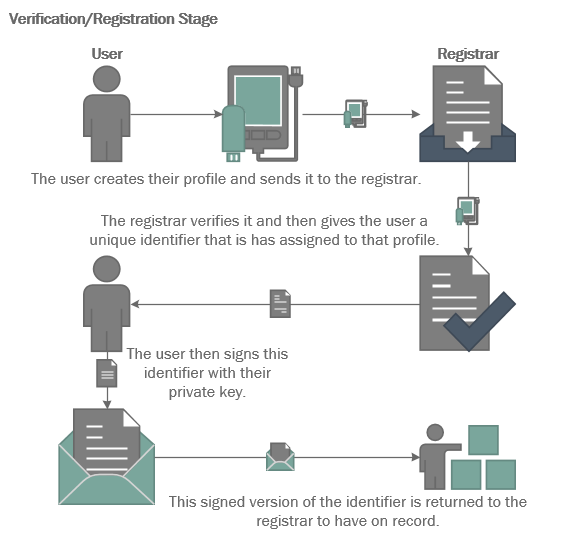
\includegraphics[width=0.75\textwidth]{verification}
    \caption{The proposed verification/registration steps.}
    \label{fig:registration}
\end{figure}

\section{Technical Considerations}

\subsection{Blockchain}

Within Blockchain technology, there are still a number of options and differing opinions on how to approach certain issues.

\par

One such key issue is which consensus algorithm to use. This consensus algorithm is what the Blockchain uses to resolve the current state of itself, such as in the case of conflicting opinions about the state of the Blockchain, and to validate transactions. This is vital due to the architecture of Blockchain technology, while anyone can add to a Blockchain we still only want one unique and final chain of transactions that we can trust. Here we will discuss two such algorithms that are used to allow the chain to do this.

\par

The first approach is the proof-of-work consensus algorithm. This is the algorithm seen in Bitcoin, where to add to the chain members must \emph{mine} a block. This mining uses a real-world resources (computational time and electricity) to solve a complex mathematical problem. As such there's no way to cheat the system by either falsification or duplicated transactions, as you must have the correct solution to the correct problem the first time it is seen. In this way the longest valid chain which has had the highest amount of work put in to it can be chosen as the correct state of the entire chain. However this brings with it certain issues, namely that each full node of the network which 'mines' and contributes in some way require substantial computing capacity proportional to the security requirements of the Blockchain. This proportional relationship is due to the fact that scarcity of the currency/transaction cost is tied directly to these real-world resources.

\par

The second is proof-of-stake. In this algorithm, instead of your computational capacity you use to contribute to the network, your stake or 'share' in the networks transactions weights your opinion on the validity of the Blockchain.

\par

MutliChain (could be its own subsection)

\subsection{User Application}

We are still currently exploring the best framework and language to provide a user-facing application for a Blockchain voting platform. The current languages being considered are JavaScript in the form of the Node.js environment and C\#.

\par

The only truly secure way to vote on Blockchain without trusting another party, is for the user to directly create their voting transaction themselves. If the user did not put their voting transaction on to the Blockchain themselves then this introduces a number of uncertainties, forcing the user to trust all intermediaries between them and their vote being placed on the Blockchain to not alter, track, or destroy that vote, and ultimately undermining the main benefits of using Blockchain technology. To allow their vote to be placed straight on to the Blockchain the end user will need to run a `Full Node'. A Full Node means that all history (blocks) of the Blockchain needs to be downloaded, as well as processing all new transactions. This means that the user will have to download and run the client on their machine, as opposed to an increasingly popular web-based application. Additionally, the size of the Blockchain is something that needs to be considered, assessed aged during the application development process. For example Bitcoin has grown to 90GB \parencite{blockchaininfosize}. The larger the number of votes, the larger the Blockchain will be.

\par

Whilst it would be desirable to have a cross-platform desktop application, given that our target audience is businesses, the majority of which use Windows [SOURCE], we have identified that it would be acceptable to produce a Windows only platform, as a prototype and an acceptable first instance of our platform. Windows accounts for almost 90\% of Desktop Operating Systems \parencite{operatingsystemstats}.

\subsection{API}

Separate from the Blockchain technologies, we have identified that an anonymous voting system will require a `Registrar' in the form of an Application Programming Interface (API). Whilst this is partially against peer-to-peer nature of Blockchain itself, and some of the methodologies surrounding Blockchain, it is necessary to provide authorisation, and limitation. Without this, anyone could vote, and they could vote as many times as they like by making multiple accounts for each vote. In order for a vote to be counted as valid, it will have to have been cast using a token that has been blindly signed by the Registrar. The registrar will also track who has been allocated tokens, and who hasn't, allowing a degree of control as to who can vote and enforcing commonly found voting regulations.

\par

Following convention, this will most likely be a web-based API. Our team does not have easy access to any Windows servers, however do have access to a few Linux servers. We plan to to write a Node.js API, interfacing with the Blockchain, and providing authority over the voting process.

\section{Final Thoughts}
\newpage
\printbibliography[heading=bibintoc]
\end{document}